\documentclass[border=0.8cm]{standalone}

\usepackage{tikz}
\usetikzlibrary{shapes.geometric, positioning, arrows.meta}

\begin{document}

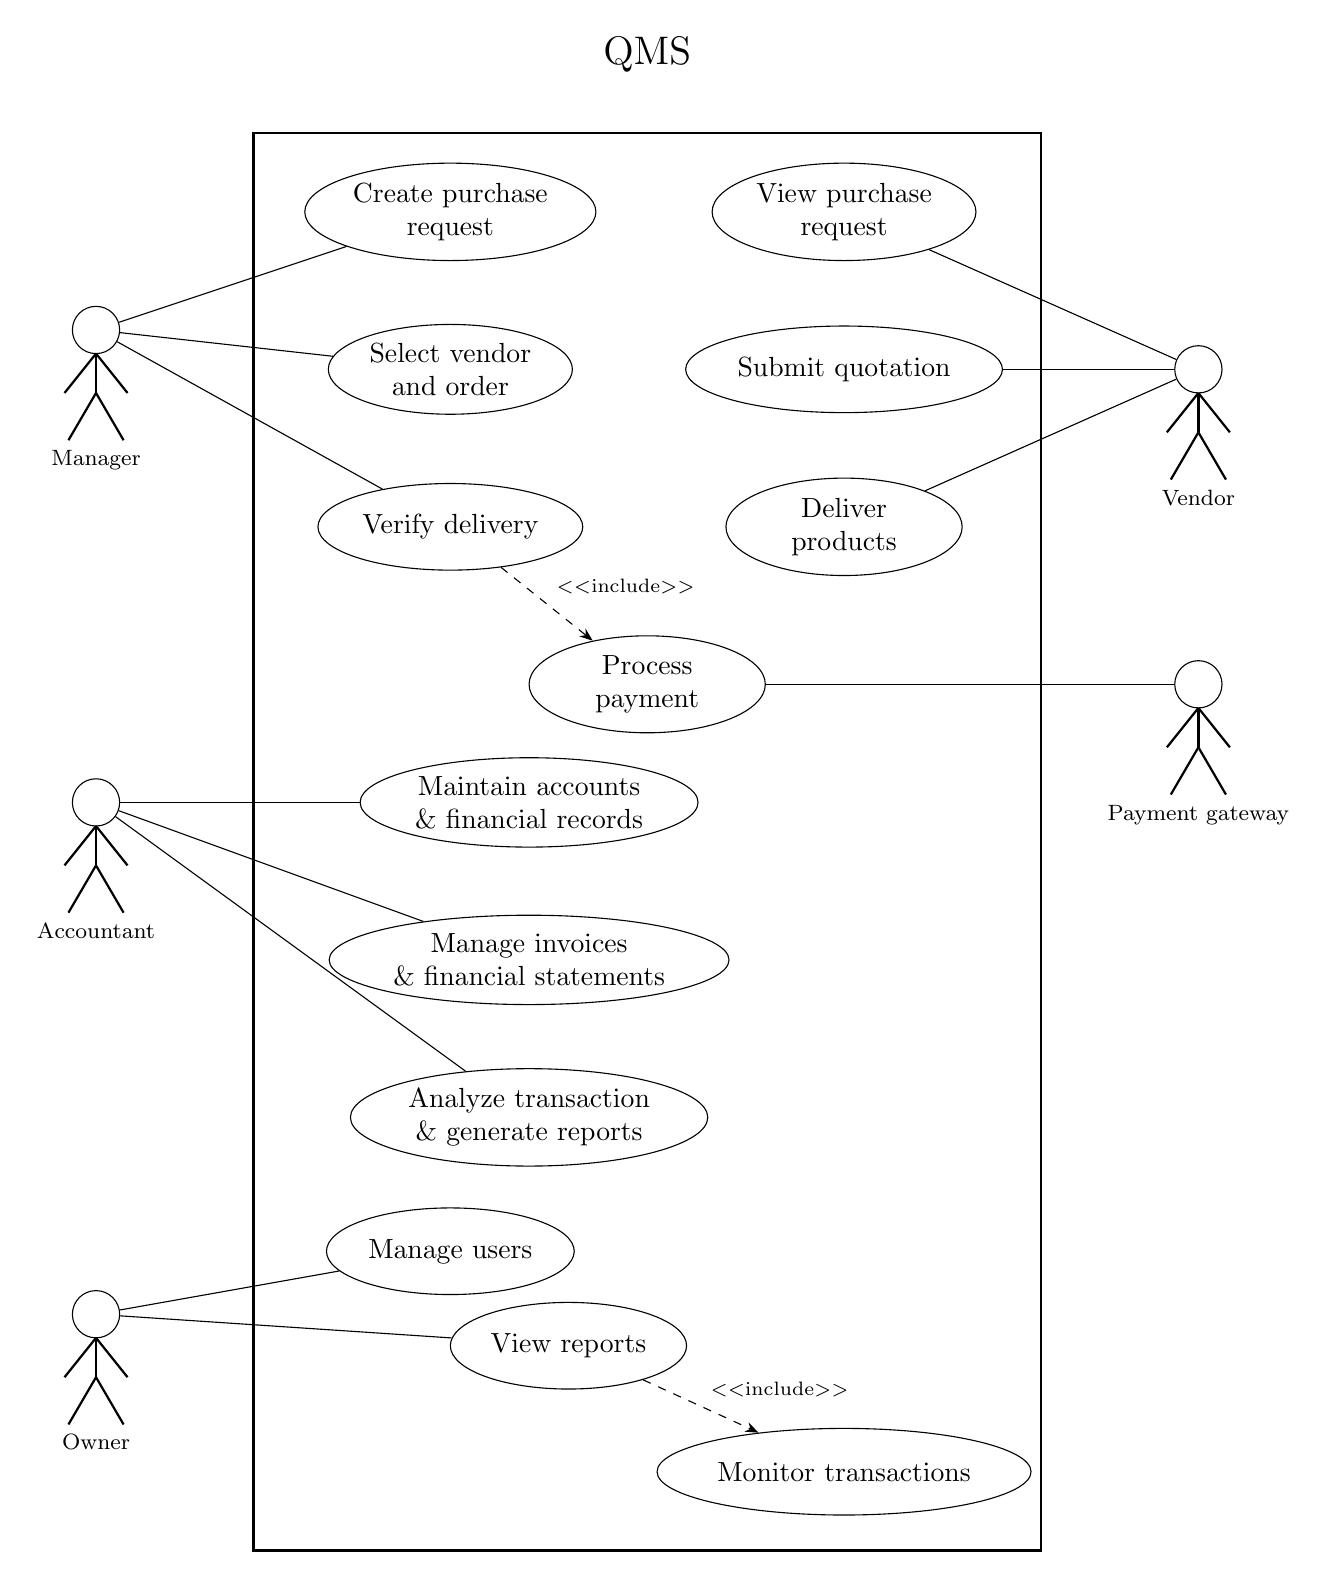
\begin{tikzpicture}[
    actor/.style={
        circle, 
        draw, 
        fill=white, 
        minimum size=6mm,
        inner sep=0pt
    },
    usecase/.style={
        ellipse, 
        draw, 
        align=center, 
        minimum width=3cm, 
        minimum height=1.1cm,
        inner sep=2pt
    },
    include/.style={
        ->,
        dashed,
        >=Stealth
    }
]

% Title
\node[font=\Large] at (5, 14.5) {QMS};

% System boundary box
\draw[thick] (0, -4.5) rectangle (10, 13.5);

% ========== ACTORS ==========

% Manager (left top)
\node[actor] (manager) at (-2, 11) {};
\draw[thick] (manager) -- ++(0, -0.8) coordinate (m1);
\draw[thick] (m1) -- ++(-0.35, -0.6);
\draw[thick] (m1) -- ++(0.35, -0.6);
\draw[thick] (manager) ++(0, -0.3) -- ++(-0.4, -0.5);
\draw[thick] (manager) ++(0, -0.3) -- ++(0.4, -0.5);
\node[below=1.1cm of manager] {\footnotesize Manager};

% Vendor (right top)
\node[actor] (vendor) at (12, 10.5) {};
\draw[thick] (vendor) -- ++(0, -0.8) coordinate (v1);
\draw[thick] (v1) -- ++(-0.35, -0.6);
\draw[thick] (v1) -- ++(0.35, -0.6);
\draw[thick] (vendor) ++(0, -0.3) -- ++(-0.4, -0.5);
\draw[thick] (vendor) ++(0, -0.3) -- ++(0.4, -0.5);
\node[below=1.1cm of vendor] {\footnotesize Vendor};

% Accountant (left middle)
\node[actor] (accountant) at (-2, 5) {};
\draw[thick] (accountant) -- ++(0, -0.8) coordinate (a1);
\draw[thick] (a1) -- ++(-0.35, -0.6);
\draw[thick] (a1) -- ++(0.35, -0.6);
\draw[thick] (accountant) ++(0, -0.3) -- ++(-0.4, -0.5);
\draw[thick] (accountant) ++(0, -0.3) -- ++(0.4, -0.5);
\node[below=1.1cm of accountant] {\footnotesize Accountant};

% Payment gateway (right middle)
\node[actor] (payment) at (12, 6.5) {};
\draw[thick] (payment) -- ++(0, -0.8) coordinate (p1);
\draw[thick] (p1) -- ++(-0.35, -0.6);
\draw[thick] (p1) -- ++(0.35, -0.6);
\draw[thick] (payment) ++(0, -0.3) -- ++(-0.4, -0.5);
\draw[thick] (payment) ++(0, -0.3) -- ++(0.4, -0.5);
\node[below=1.1cm of payment] {\footnotesize Payment gateway};

% Owner (left bottom)
\node[actor] (owner) at (-2, -1.5) {};
\draw[thick] (owner) -- ++(0, -0.8) coordinate (o1);
\draw[thick] (o1) -- ++(-0.35, -0.6);
\draw[thick] (o1) -- ++(0.35, -0.6);
\draw[thick] (owner) ++(0, -0.3) -- ++(-0.4, -0.5);
\draw[thick] (owner) ++(0, -0.3) -- ++(0.4, -0.5);
\node[below=1.1cm of owner] {\footnotesize Owner};

% ========== USE CASES - MANAGER SECTION ==========

\node[usecase] (create) at (2.5, 12.5) {Create purchase\\request};
\node[usecase] (select) at (2.5, 10.5) {Select vendor\\and order};
\node[usecase] (verify) at (2.5, 8.5) {Verify delivery};

% ========== USE CASES - VENDOR SECTION ==========

\node[usecase] (view) at (7.5, 12.5) {View purchase\\request};
\node[usecase] (submit) at (7.5, 10.5) {Submit quotation};
\node[usecase] (deliver) at (7.5, 8.5) {Deliver\\products};

% ========== USE CASES - PAYMENT PROCESS ==========

\node[usecase] (process) at (5, 6.5) {Process\\payment};

% ========== USE CASES - ACCOUNTANT SECTION ==========

\node[usecase] (maintain) at (3.5, 5) {Maintain accounts\\ \& financial records};
\node[usecase] (manageinv) at (3.5, 3) {Manage invoices\\ \&  financial statements};
\node[usecase] (analyze) at (3.5, 1) {Analyze transaction\\ \&  generate reports};

% ========== USE CASES - OWNER SECTION (WITH EQUAL SPACING) ==========

\node[usecase] (manageuser) at (2.5, -0.7) {Manage users};

\node[usecase] (viewreport) at (4, -1.9) {View reports};

\node[usecase] (monitor) at (7.5, -3.5) {Monitor transactions};

% ========== CONNECTIONS - MANAGER ==========

\draw (manager) -- (create);
\draw (manager) -- (select);
\draw (manager) -- (verify);

% ========== CONNECTIONS - VENDOR ==========

\draw (vendor) -- (view);
\draw (vendor) -- (submit);
\draw (vendor) -- (deliver);

% ========== CONNECTIONS - ACCOUNTANT ==========

\draw (accountant) -- (maintain);
\draw (accountant) -- (manageinv);
\draw (accountant) -- (analyze);

% ========== CONNECTIONS - OWNER ==========

\draw (owner) -- (manageuser);
\draw (owner) -- (viewreport);

% ========== CONNECTIONS - PAYMENT GATEWAY ==========

\draw (payment) -- (process);

% ========== INCLUDE RELATIONSHIPS ==========

\draw[include] (verify) -- (process) node[midway, above right, font=\scriptsize] {$<<$include$>>$};

\draw[include] (viewreport) -- (monitor) node[midway, above right, font=\scriptsize]{$<<$include$>>$};

\end{tikzpicture}

\end{document}
